\chapter{Diseño e implementación} % Main chapter title

\label{Chapter3} % Change X to a consecutive number; for referencing this chapter elsewhere, use \ref{ChapterX}

\definecolor{mygreen}{rgb}{0,0.6,0}
\definecolor{mygray}{rgb}{0.5,0.5,0.5}
\definecolor{mymauve}{rgb}{0.58,0,0.82}

%%%%%%%%%%%%%%%%%%%%%%%%%%%%%%%%%%%%%%%%%%%%%%%%%%%%%%%%%%%%%%%%%%%%%%%%%%%%%
% parámetros para configurar el formato del código en los entornos lstlisting
%%%%%%%%%%%%%%%%%%%%%%%%%%%%%%%%%%%%%%%%%%%%%%%%%%%%%%%%%%%%%%%%%%%%%%%%%%%%%
\lstset{ %
  backgroundcolor=\color{white},   % choose the background color; you must add \usepackage{color} or \usepackage{xcolor}
  basicstyle=\footnotesize,        % the size of the fonts that are used for the code
  breakatwhitespace=false,         % sets if automatic breaks should only happen at whitespace
  breaklines=true,                 % sets automatic line breaking
  captionpos=b,                    % sets the caption-position to bottom
  commentstyle=\color{mygreen},    % comment style
  deletekeywords={...},            % if you want to delete keywords from the given language
  %escapeinside={\%*}{*)},          % if you want to add LaTeX within your code
  %extendedchars=true,              % lets you use non-ASCII characters; for 8-bits encodings only, does not work with UTF-8
  %frame=single,	                % adds a frame around the code
  keepspaces=true,                 % keeps spaces in text, useful for keeping indentation of code (possibly needs columns=flexible)
  keywordstyle=\color{blue},       % keyword style
  language=[ANSI]C,                % the language of the code
  %otherkeywords={*,...},           % if you want to add more keywords to the set
  numbers=left,                    % where to put the line-numbers; possible values are (none, left, right)
  numbersep=5pt,                   % how far the line-numbers are from the code
  numberstyle=\tiny\color{mygray}, % the style that is used for the line-numbers
  rulecolor=\color{black},         % if not set, the frame-color may be changed on line-breaks within not-black text (e.g. comments (green here))
  showspaces=false,                % show spaces everywhere adding particular underscores; it overrides 'showstringspaces'
  showstringspaces=false,          % underline spaces within strings only
  showtabs=false,                  % show tabs within strings adding particular underscores
  stepnumber=1,                    % the step between two line-numbers. If it's 1, each line will be numbered
  stringstyle=\color{mymauve},     % string literal style
  tabsize=2,	                   % sets default tabsize to 2 spaces
  title=\lstname,                  % show the filename of files included with \lstinputlisting; also try caption instead of title
  morecomment=[s]{/*}{*/}
}

En éste capítulo se describe la estructura de la solución adoptada y el funcionamiento del hardware, software y firmware desarrollado específicamente para el cumplimiento de los requerimientos del sistema.

\section{Solución adoptada}

En base a los requerimientos enumerados en el capítulo 2, se desarrolló un sistema utilizando las tecnologías indicadas en la tabla [\ref{tab:solucionadoptada}].

\begin{table}[h]
	\centering
	\caption[Solución adoptada]{Tecnologías utilizadas en el desarrollo del sistema}
	\begin{tabular}{l m{4.5cm} m{4.5cm}}    
		\toprule
		\textbf{}  					& \textbf{Nodo}     				& \textbf{Gateway}	\\
		\midrule
		Aplicación 					& \ Firmware en C/C++				& \ Firmware en C/C++ y software en Python. \\
		Sistema operativo	 		& \ No corresponde 					& \ Linux\\
		Hardware		 			& \ ESP32(Xtensa LX6) 				& \ Raspberry Pi 3 (Cortex-A53) y ESP32 (Xtensa LX6)\\
		\bottomrule
		\hline
	\end{tabular}
	\label{tab:solucionadoptada}
\end{table}

Se implementó el hardware del nodo en una placa de circuito impreso de diseño específico, que se describirá en la sección \ref{sec:nodos}. Ésta contiene un microcontrolador de arquitectura MIPS({\textit{Microprocessor without Interlocked Pipeline Stages}}) de 32 bits. Cada nodo posee un circuito integrado de comunicación LoRa con su respectiva antena, sensores y actuadores, ésta permanece a la espera de recepción de comandos, conforme al protocolo propietario desarrollado.

Además se utilizó una Raspberry Pi como gateway descrito en la seccion \ref{sec:gateway}, a la cual se le conecta un hardware similar al nodo para utilizarlo como transceptor LoRa. La Raspberry Pi corre el sistema operativo Linux en la tarjeta microSD. También se desarrolló una aplicación en Python como {\textit{Backend}} de la interfaz web creada en Node-Red.


%----------------------------------------------------------------------------------------
%	SECTION 1
%----------------------------------------------------------------------------------------
\section{Arquitectura de funcionamiento}

En ésta sección se explica la arquitectura utilizada para la comunicación inalámbrica del sistema.
Se toma como referencia la arquitectura distribuida descrita en la sección \ref{sec:arquitecturadedomotica}. Ésta indica que la toma de decisiones por parte del sistema se encuentra en todos los dispositivos, no solo en uno central.
En la figura [\ref{fig:diagramadesecuencia}] se muestra el diagrama de secuencia del sistema. Éste se encuentra montado sobre una red inalámbrica local que utiliza el protocolo LoRa entre gateway y los nodos.

\begin{figure}[ht!]
	\centering
	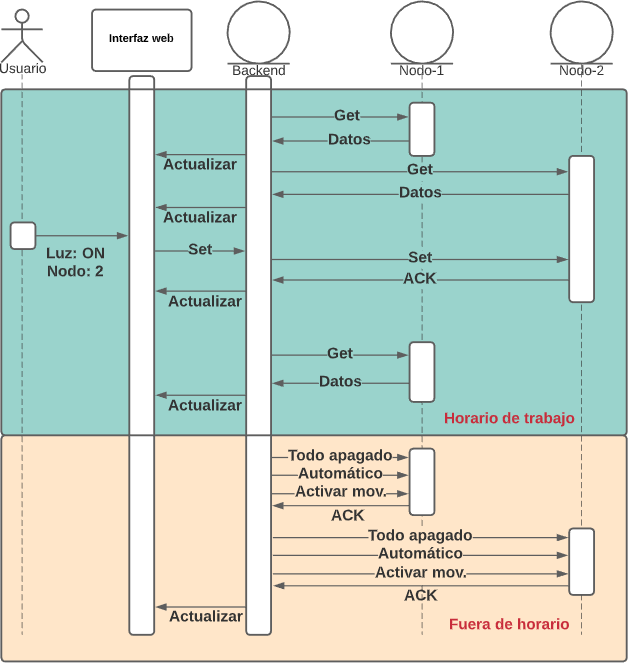
\includegraphics[width=0.8\textwidth]{./Figures/diagramadesecuencia.png}
	\caption{Diagrama de secuencia del sistema.}
	\label{fig:diagramadesecuencia}
\end{figure}

La arquitectura utilizada posee dos acciones posibles: {\textit{Set}} y {\textit{Get}}. El objetivo de esta arquitectura es la de poder recibir datos con el comando {\textit{Get}} y configurar parámetros con el comando {\textit{Set}}.
En este sistema, cuando existe un nodo o una red de nodos, el gateway se encuentra enviando el comando {\textit{Get}} a cada nodo en intervalos de 20 segundos. Ésto permite que la interfaz web se actualice constantemente. Al no ser un sistema crítico no se necesitan tiempos de respuesta rápidos por lo que 20 segundos es un tiempo prudente.
El nodo no tiene permitido enviar datos sin antes haber recibido el comando {\textit{Get}}, la unica excepción es cuando está en modo automático y tiene activado el sensor de movimiento.


\section{Nodos}
\label{sec:nodos}

El nodo es el dispositivo del sistema del cual se extrae la información de los sensores. Los actuadores se utilizan para generar cambios en dispositivos externos al sistema inalámbrico como ser un aire acondicionado. En esta sección se explicara el hardware y parte del firmware del nodo.

\subsection{Hardware}

El hardware del nodo contiene los siguientes componentes:

\begin{enumerate}
\item Una fuente AC-DC de 220v a 5v (ver figura[\ref{fig:esquematico1}]).
\item Sensor de temperatura y humedad (ver figura[\ref{fig:esquematico2}]).
\item Modulo Heltec LoRa v2 con antena adaptada a 915MHz (ver figura[\ref{fig:esquematico3}]).
\item Circuito de leds infrarrojos (ver figura[\ref{fig:esquematico4}]).
\item Circuito relay (ver figura[\ref{fig:esquematico5}]).
\item Circuito de pulsadores (ver figura[\ref{fig:esquematico6}]).
\item Circuito de leds indiciadores (ver figura[\ref{fig:esquematico7}]).
\end{enumerate}

En la figura [\ref{fig:esquematico1}] se tiene el circuito de la fuente. Se decidió buscar en el mercado una fuente compacta y pequeña debido al tamaño final que debe tener el producto. Se utilizó la fuente compacta HLK-PM01 de la empresa Hi-Link.

\begin{figure}[h!]
	\centering
	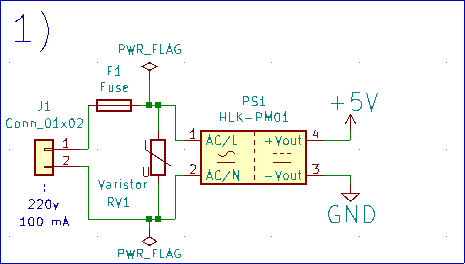
\includegraphics[width=0.6\textwidth]{./Figures/esquematico1.png}
	\caption{Circuito de fuente AC-DC.}
	\label{fig:esquematico1}
\end{figure}

En la figura [\ref{fig:esquematico2}] se muestra el circuito del sensor de temperatura y humedad. El sensor es el conocido DHT11 que tiene un rango de temperatura de 0 a 50 ºC con 5\% de precisión y un rango de humedad de 20 al 80 \% con una precisión del 5\%.

\begin{figure}[h!]
	\centering
	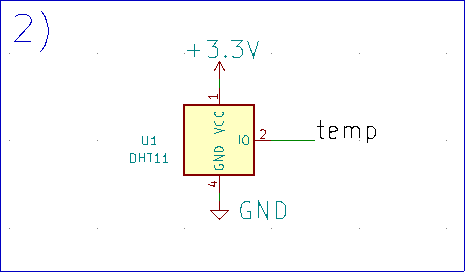
\includegraphics[width=0.6\textwidth]{./Figures/esquematico2.png}
	\caption{Circuito de sensor de temperatura.}
	\label{fig:esquematico2}
\end{figure}

En la figura [\ref{fig:esquematico3}] se ve el circuito de conectores que ofician de zócalo para conectar el modulo externo Heltec LoRa v2. Éste módulo fue elegido debido a que ofrece un microcontrolador ESP32 de arquitectura Tensilica Xtensa LX6 de 32bits por lo que se utiliza como controlador principal del nodo, además posee un display OLED y el circuito integrado {\textit{SX1276}} de la empresa Semtech, con conector Hirose U.FL para antenas miniatura de RF de hasta 6 GHz.

\begin{figure}[h!]
	\centering
	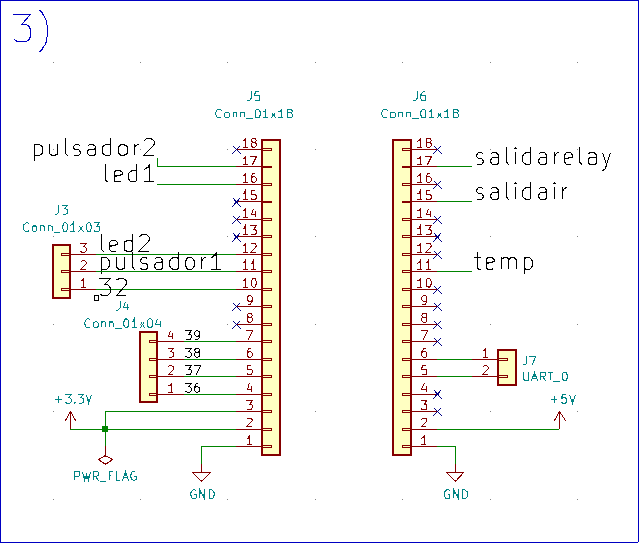
\includegraphics[width=0.6\textwidth]{./Figures/esquematico3.png}
	\caption{Conectores para el modulo Heltec LoRa v2.}
	\label{fig:esquematico3}
\end{figure}

En la figura [\ref{fig:esquematico4}] se ve un circuito típico para el uso de leds habilitado por transistor. Se utilizaron dos leds debido a que en las pruebas de alcance se obtuvo mayor rendimiento del haz infrarrojo con respecto a los aires acondicionados. El led infrarrojo es el actuador para el encendido y apagado de los aires acondicionados.

\begin{figure}[h!]
	\centering
	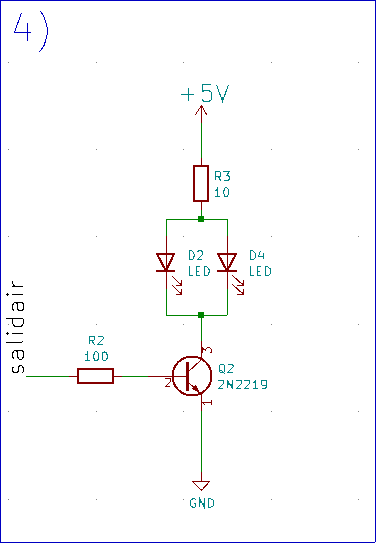
\includegraphics[width=0.4\textwidth]{./Figures/esquematico4.png}
	\caption{Circuito de leds infrarrojos.}
	\label{fig:esquematico4}
\end{figure}

En la figura [\ref{fig:esquematico5}] se tiene un circuito típico de relay con su respectivo conector de salida. El relay es el actuador para el encendido y apagado de la luz.

\begin{figure}[h!]
	\centering
	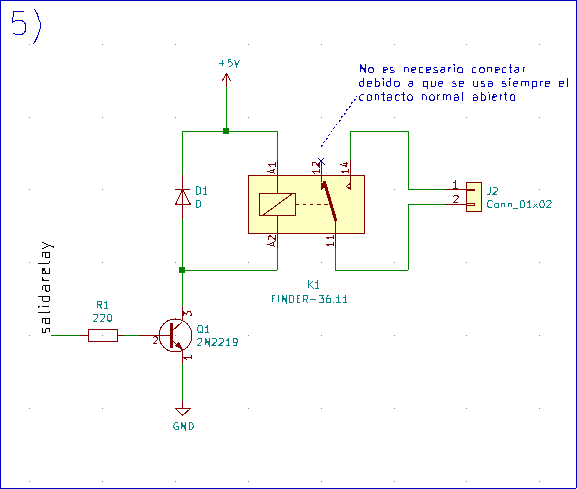
\includegraphics[width=0.6\textwidth]{./Figures/esquematico5.png}
	\caption{Circuito de relay.}
	\label{fig:esquematico5}
\end{figure}

En la figura [\ref{fig:esquematico6}] se muestra el circuito de los pulsadores, éstos son el pulsador de {\textit{Modo}} que se utiliza para sincronizar el nodo con el gateway y además para cambiar el modo de manual a automático, y el pulsador para encendido y apagado de la luz.

\begin{figure}[h!]
	\centering
	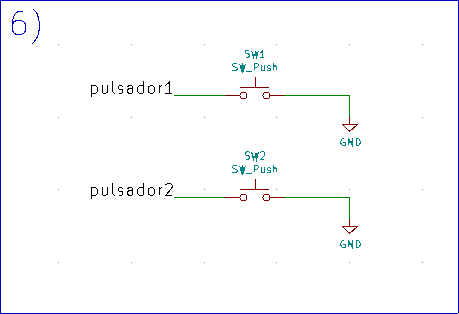
\includegraphics[width=0.5\textwidth]{./Figures/esquematico6.png}
	\caption{Circuito de pulsadores.}
	\label{fig:esquematico6}
\end{figure}

En la figura [\ref{fig:esquematico7}] se muestra el circuito de leds indicadores, se utilizan para {\textit{debugging}} del sistema.

\begin{figure}[h!]
	\centering
	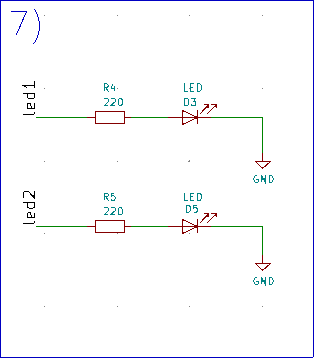
\includegraphics[width=0.4\textwidth]{./Figures/esquematico7.png}
	\caption{Circuito de leds indicadores.}
	\label{fig:esquematico7}
\end{figure}

La imagen renderizada de la placa de circuito impreso desarrollada en la herramienta libre Kicad, se muestra en la figura [\ref{fig:pcb1}].

\begin{figure}[h!]
	\centering
	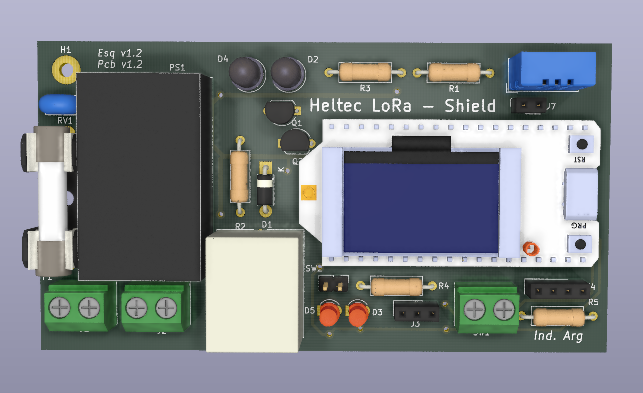
\includegraphics[width=0.6\textwidth]{./Figures/pcb1.png}
	\caption{Render de placa de circuito impreso.}
	\label{fig:pcb1}
\end{figure} 

En la figura [\ref{fig:pcb2}] se puede ver la imagen de la PCB terminada. Ésta es una PCB de doble capa, realizada de forma casera con el método de insolación ultravioleta.

\begin{figure}[h!]
	\centering
	\includegraphics[width=0.6\textwidth]{./Figures/pcb2.png}
	\caption{Placa de circuito impreso.}
	\label{fig:pcb2}
\end{figure} 

\subsection{Firmware}

La arquitectura del firmware se diseñó teniendo en cuenta algunos patrones de diseño de arquitectura y conceptos de programación orientada a objetos en C/C++.
El patrón de diseño de arquitectura utilizado fue: Control ambiental. Porque se tiene un proceso de control de la planta mediante sensores y actuadores, además se tiene un proceso de despliegue que es la muestra de datos en la pantalla OLED y el reporte de los cambios al gateway.
Para el desarrollo del firmware se utilizó la biblioteca que provee el fabricante del módulo Heltec LoRa, éste provee los drivers de la siguiente lista:

\begin{itemize}
\item Display OLED 128x64.
\item Protocolo LoRa.
\end{itemize}

Además se utilizó una librería creada para el uso de infrarrojos con el microcontrolador ESP32, con el objetivo de agilizar el desarrollo ya que existe una gran variedad de aires acondicionados y protocolos muy variados. Se encontró que la librería provee 92 protocolos, es decir, 92 dispositivos distintos a los cuales se los puede manipular con infrarrojo. Si bien la API de la empresa {\textit{Espressif}} (ESP-IDF), está desarrollada completamente sobre el sistema operativo de tiempo real freeRTOS. Se utilizó como API principal la de Arduino debido a que el sistema no necesita ser de tiempo real, ésta provee soluciones que agilizan el desarrollo en este tipo de proyectos.

El firmware posee un arquitectura en capas, esto permite la separación de las partes que componen el sistema. En la figura [\ref{fig:capas}] se pueden ver las capas que componen el sistema.

\begin{figure}[h!]
	\centering
	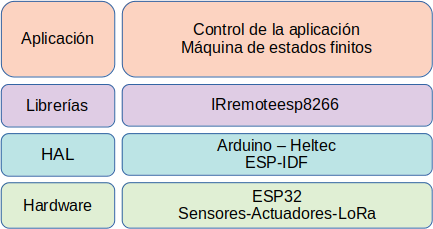
\includegraphics[width=0.7\textwidth]{./Figures/capas.png}
	\caption{Arquitectura en capas del firmware del nodo.}
	\label{fig:capas}
\end{figure}

El diagrama de flujo del sistema es el que se muestra en la figura [\ref{fig:diagramaflujo}].

\begin{figure}[h!]
	\centering
	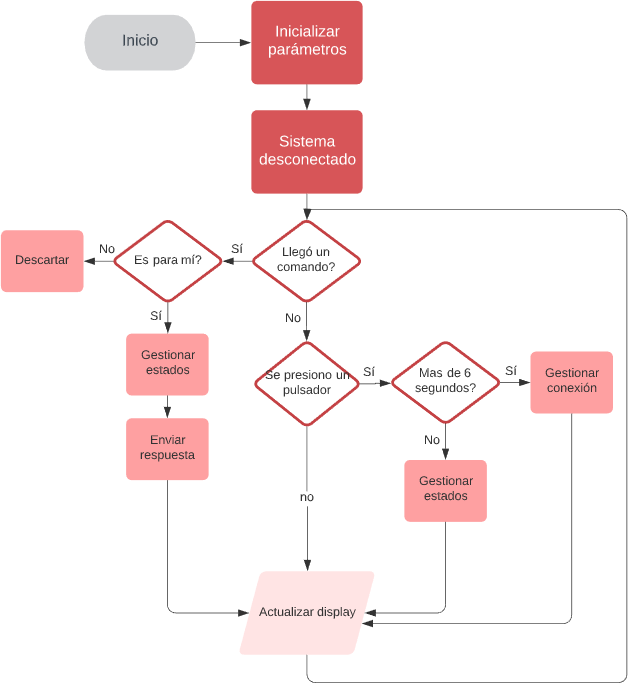
\includegraphics[width=0.9\textwidth]{./Figures/diagramaflujo.png}
	\caption{Diagrama de flujo del nodo.}
	\label{fig:diagramaflujo}
\end{figure}

La estructura de inicialización y el loop principal del sistema se puede ver en la sección de código [\ref{cod:main}].

\begin{lstlisting}[label=cod:main,caption=Estructura principal de código. Archivo {\textit{main.cpp}} ]  % Start your code-block

#include <Arduino.h>
#include "main.h"

void setup()
{
  Serial.begin(115200);
  fsm_machine_init(&serialdata, &control, &lora_node);
}

void loop()
{
  fsm_machine_control(&serialdata, &control, &lora_node);
  fsm_button_check(&control, &serialdata, &lora_node);
}

\end{lstlisting}

Dentro del archivo de funciones de la maquina de estados finitos ({\textit{fsm.cpp}}), se tienen dos funciones principales. Éstas funciones se pueden ver en la sección de código [\ref{cod:fsm}].

\begin{lstlisting}[label=cod:fsm,caption=Funciones de la maquina de estados finitos]  % Start your code-block

void    fsm_machine_init(serialdata_t *serialdata,control_t *control,lora_node_t *lora_node);

void    fsm_machine_control(serialdata_t *serialdata,control_t *control,lora_node_t *lora_node);

\end{lstlisting}

La primera se encarga de inicializar todos los parámetros necesarios para que el sistema funcione. En la siguiente lista se ponen en conocimiento los parámetros inicializados antes de empezar el loop principal:

\begin{itemize}
\item Display OLED y tamaño de fuente.
\item Los pines de entrada y salida:
\begin{itemize}
\item Salida a relay.
\item Salida a leds infrarrojos.
\item Entrada de señal del sensor de temperatura y humedad.
\item Salida a leds indicadores.
\item Entrada de pulsadores.
\end{itemize}
\item Estados predeterminados del sistema ante un reset.
\item Parámetros del protocolo LoRa como ser la frecuencia de 915MHz.
\end{itemize}

La segunda función tiene como objetivo controlar todos los estados del sistema y actualizarlos cada vez que llegue un comando o que la temperatura se actualice. Se utilizaron tres estructuras principales que se listan a continuación:

\begin{itemize}
\item Control
\item Lora node
\item Serial data
\end{itemize}

La primera se muestra en la sección de código [\ref{cod:control}].

\begin{lstlisting}[label=cod:control,caption=Estructura de control del nodo] 

typedef struct {
    general_states_s    generalStates;
    working_states_s    workingStates;
    relay_states_s      relayStates;
    mov_states_s        movStates;
    a_conditioner_s     aConditioner;
    pin_struct_t        pin;
    dht_t               dhtVal;
    aa_struct_t         aa_conf;
    uint16_t            nodeId;
}control_t;

\end{lstlisting}

Los primeros 5 elementos de la estructura corresponden a variables del tipo {\textit{ENUM}} y cada una puede tomar los estados que se muestran en la tabla [\ref{tab:estados}]:

\begin{table}[h]
	\centering
	\caption[Estados de periféricos y variables del nodo]{Estados de periféricos y variables del nodo}
	\begin{tabular}{l c c c c}    
		\toprule
		\textbf{generalStates}		& \textbf{workingStates}	& \textbf{relayStates}		& \textbf{movStates}	& \textbf{aConditioner}		\\
		\midrule
		Automático					& \ Working 				& \ ON						& \ Activado			& \ ON							\\
		Manual 						& \ Not working				& \ OFF						& \ Desactivado			& \ OFF							\\
		\bottomrule
		\hline
	\end{tabular}
	\label{tab:estados}
\end{table}

El problema que se tiene es que el gateway debe permitir una gran cantidad de nodos, tantos como sea posible y eso requiere que cada nodo tenga su propio numero de identificación con el objetivo de que no existan ambigüedades a la hora de la comunicación entre un nodo y un gateway, es decir, para que el gateway identifique a quien enviar y de quien recibe los paquetes.
Se optó por utilizar un ID que se crea en cada nodo automáticamente y es único. La solución fue usar la dirección MAC de 64 bits que tiene cada microcontrolador ESP32 y acortarla a 16 bits debido a que con esa cantidad es suficiente para un sistema de éste tipo. Ésta variable es la última de la estructura, es un {\textit{unsigned int 16}} llamado {\textit{nodeId}}. 

La segunda estructura utilizada es la que se muestra en la sección de código [\ref{cod:lora}]. En esta estructura se tiene un flag de conexión que cambia si el sistema se encuentra conectado o desconectado, nodeChar es un array donde se guarda la palabra NODE:ID y que luego sirve para comparar con comandos recibidos, finalmente stateNode es una variable del tipo {\textit{ENUM}} que dentro tiene los estados que se listan en la tabla [\ref{tab:lora}].

\begin{lstlisting}[label=cod:lora,caption=Estructura de control del protocolo LoRa] 

typedef struct lora_node_t{
    bool            loraConnectionFlag;
    char            nodeChar[20];
    lora_state_s    stateNode;
}lora_node_t;

\end{lstlisting}

\begin{table}[h]
	\centering
	\caption[Estados de conexión]{Estados de la variable stateNode.}
	\begin{tabular}{l}    
		\toprule
		\textbf{stateNode}		\\
		\midrule
		Conectado				\\
		Desconectado			\\
		Alarma					\\
		\bottomrule
		\hline
	\end{tabular}
	\label{tab:lora}
\end{table}

La estructura {\textit{serialdata}} se puede ver en la sección de código [\ref{cod:serialdata}]. Ésta estructura fue muy importante en la primera etapa de desarrollo del sistema porque se utilizó para hacer debugging a través del puerto serie propio del nodo, antes de tener una conexión inalámbrica a través de LoRa e inclusive antes de tener un gateway que se comunique con éste. Contiene a todos los comandos que deben ser comparados por el nodo cuando recibe datos de forma inalámbrica, por lo cual no se descartó su uso.

\begin{lstlisting}[label=cod:serialdata,caption=Estructura de control de comandos por el puerto serie.] 

typedef struct serialdata_t
{
   bool                newData;
   char                *startMarker;
   char                *endMarker;
   char                rc;
   char                receivedChars[NUMCHARS];
   bool                configFlag;
   bool                getDataFlag;
   uint16_t            nodeId;
   bool                nodeConection;
   commands_c          commands;
} serialdata_t;

\end{lstlisting}

Finalmente se explica la función {\textit{fsm button check}} que se ve en la sección de código [\ref{cod:main}]. Ésta función tiene como objetivo hacer un polling de los pines de entrada de los pulsadores e implementa funciones de antirebote para verificar los pines.


\section{Gateway}
\label{sec:gateway}

El gateway es el dispositivo del sistema que maneja la información de todos los nodos y la guarda en base de datos. Se encarga de preguntar a cada nodo el estado de sus periféricos y sensores para así actualizar la base de datos, también realiza la gestión de conexión con los nodos y envío de comandos para setear parámetros. En esta sección se explicará el hardware y software del gateway.

\subsection{Hardware}

El hardware del gateway contiene los siguientes componentes:

\begin{enumerate}
\item Raspberry Pi 3. Figura [\ref{fig:raspberry}].
\item Modulo Heltec LoRa v2 con antena adaptada a 915MHz. Figura [\ref{fig:helteclora}].
\end{enumerate}

En la figura [\ref{fig:raspberry}] se puede ver el primer componente listado anteriormente. La Raspberry es un ordenador de placa única y de bajo costo, éstos fueron los motivos por el cual se la eligió, además de tener mucho soporte por la comunidad.
En éste proyecto se encarga de gestionar la información que envían los nodos y tenerla disponible en la base de datos para actualizar la interfaz web que se detallará en la sección [\ref{sec:interfaz}].

\begin{figure}[h!]
	\centering
	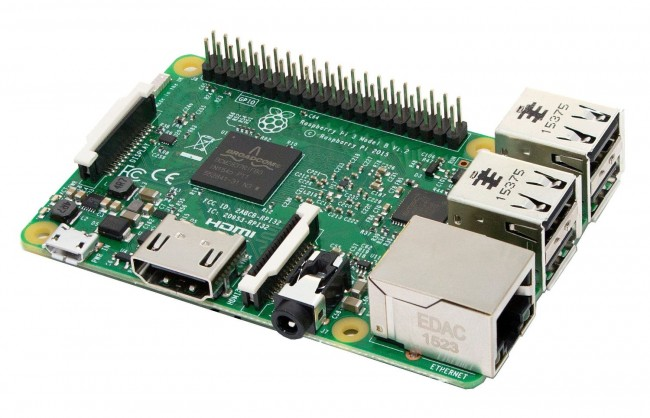
\includegraphics[width=0.55\textwidth]{./Figures/raspberry.jpg}
	\caption{Raspberry Pi 3.}
	\label{fig:raspberry}
\end{figure}

El componente número dos de la lista es el módulo que se ve en la figura [\ref{fig:helteclora}]. Éste módulo creado por la empresa Heltec es igual al que se utiliza en el nodo con la diferencia de que el firmware es completamente distinto. Éste gestiona la UART que incorpora, se encarga de recibir y enviar comandos a través del protocolo LoRa utilizando el circuito integrado {\textit{SX1276}} de la empresa Semtech, y funciona como un periférico de la Raspberry.

\begin{figure}[h!]
	\centering
	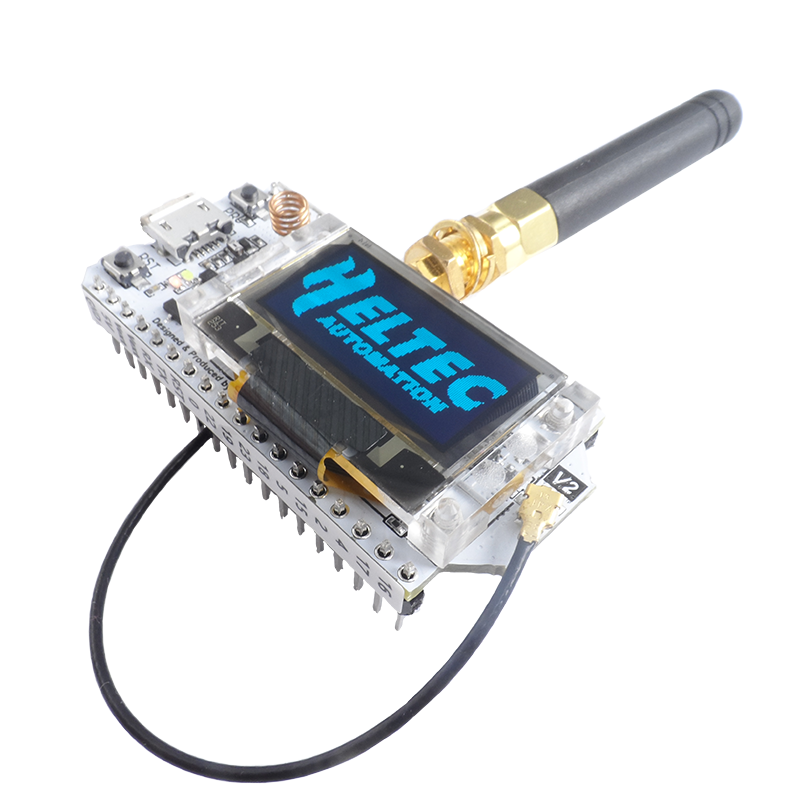
\includegraphics[width=0.35\textwidth]{./Figures/helteclora.png}
	\caption{Módulo Heltec LoRa v2.}
	\label{fig:helteclora}
\end{figure}

Los dispositivos listados se conectan a través de un cable USB como el de la figura [\ref{fig:usb}].

\begin{figure}[h!]
	\centering
	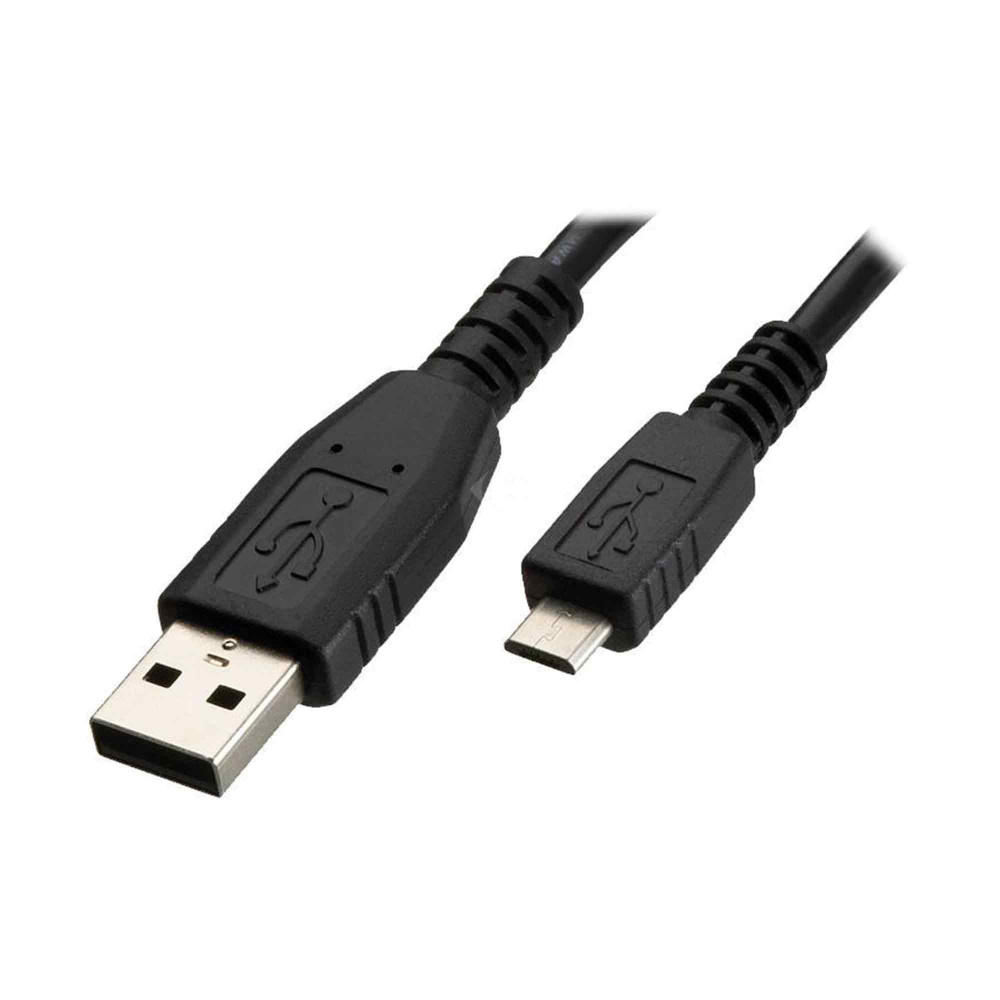
\includegraphics[width=0.25\textwidth]{./Figures/usb.jpg}
	\caption{Cable USB.}
	\label{fig:usb}
\end{figure}


\subsection{Software y Firmware}

El software desarrollado para la Raspberry pi 3 fue escrito en Python que es un lenguaje de programación interpretado cuya filosofía hace hincapié en la legibilidad de su código. Se trata de un lenguaje de programación multiparadigma, ya que soporta orientación a objetos, programación imperativa y, en menor medida, programación funcional ~\cite{pythonweb}. A continuación se listan los procesos que gestiona el software desarrollado.

\begin{enumerate}
\item Base de datos creada en SQLITE.
\item Archivos .txt y .csv utilizados para el {\textit{Backend}}.
\item Puerto serie conectado al transceptor LoRa.
\item Comandos enviados y recibidos.
\end{enumerate}

El sistema se inicializa verificando la conexión USB con el transceptor LoRa. Si la conexión no existe, el proceso se cierra automáticamente. En el caso de que la conexión sea satisfactoria el proceso crea hilos que gestionan los siguientes ítems:

\begin{itemize}
\item Envío de comando {\textit{Get}} a los nodos, éste comando se utiliza para que el nodo responda con información acerca de sus sensores y actuadores, todo ésto lo hace utilizando la información de la base de datos creada al agregar nuevos nodos.
\item Recepción de datos por parte de los nodos, actualizando la base de datos en SQLITE.
\item Gestión de los archivos que se crean al interactuar con la interfaz web.
\end{itemize}

El firmware del transceptor LoRa es muy simple. Su tarea es la de transmitir los comandos que recibe por la UART a través del protocolo LoRa y luego si recibe algo a través de LoRa, lo retransmite por la UART. El diagrama de flujos es el que se muestra en la figura [\ref{fig:diagramagateway}]. El firmware fue escrito en C/C++.

\begin{figure}[h!]
	\centering
	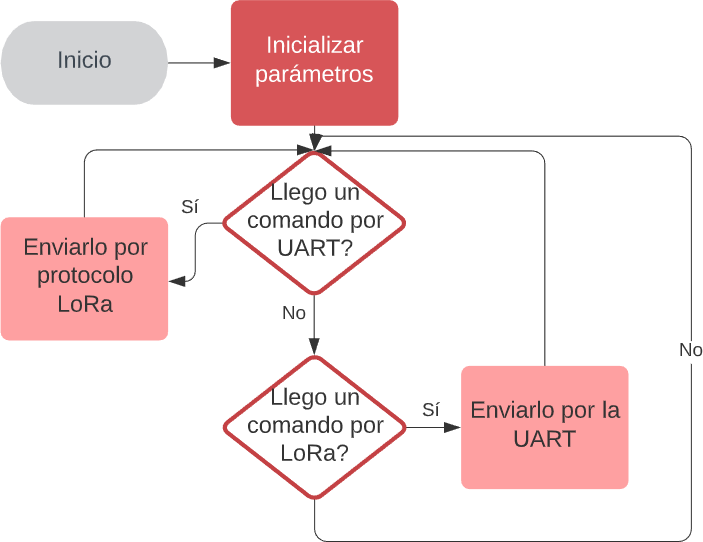
\includegraphics[width=0.7\textwidth]{./Figures/diagramagateway.png}
	\caption{Diagrama de flujo del transceptor.}
	\label{fig:diagramagateway}
\end{figure}


\section{Interfaz web}
\label{sec:interfaz}

La interfaz de usuario es el medio por el cual el usuario puede comunicarse con una máquina, equipo, computadora o dispositivo, y comprende todos los puntos de contacto entre el usuario y el equipo.
En este trabajo se comenzó a utilizar {\textit{Flask}} que es un framework minimalista escrito en Python que permite crear aplicaciones web rápidamente, pero surgieron problemas por la complejidad de las funcionalidades que se le tuvo que dar a la interfaz. Por ello, se decidió utilizar finalmente {\textit{Node-red}} que es una herramienta de programación visual, que permite el rápido desarrollo de un {\textit{dashboard}} para el sistema, de manera que agilizó el proceso completamente.
Se creó un {\textit{dashboard}} intuitivo para el uso del usuario, que contiene las siguientes pestañas:

\begin{itemize}
\item Información
\item Configuración
\item Reset
\end{itemize}

La pestaña de información se puede ver en la figura [\ref{fig:informacion}]. En ésta pestaña se tiene la información de los nodos como sensores y estados, y también botones y solapa de elección de protocolo del aire acondicionado para cada nodo. A continuación se detalla de manera mas precisa las funcionalidades.

\begin{enumerate}
\item Encendido y apagado de luz.
\item Encendido y apagado de aire acondicionado.
\item Elección del protocolo del aire acondicionado.
\item Elección de modo manual o automático.
\item Activar o desactivar movimiento.
\end{enumerate}

\begin{figure}[h!]
	\centering
	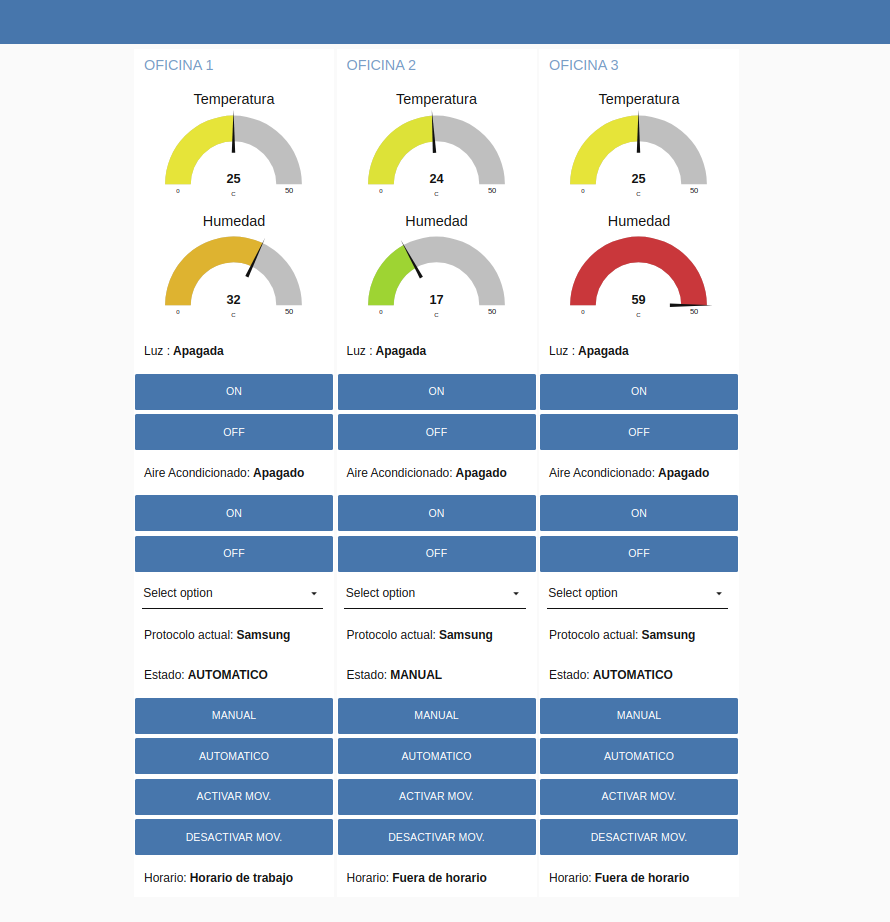
\includegraphics[width=1\textwidth]{./Figures/informacion.png}
	\caption{Pestaña de información de la interfaz web.}
	\label{fig:informacion}
\end{figure}

La pestaña de configuración se puede ver en la figura [\ref{fig:configuracion}]. Se detallan las funcionalidades de dicha pestaña en la siguiente lista.

\begin{enumerate}
\item Agregar un nodo nuevo al sistema y base de datos.
\item Elegir el horario de entrada del personal del edificio.
\item Elegir el horario de salida del personal del edificio.
\item Habilitar o deshabilitar el uso de los horarios de entrada y salida.
\end{enumerate}

\begin{figure}[h!]
	\centering
	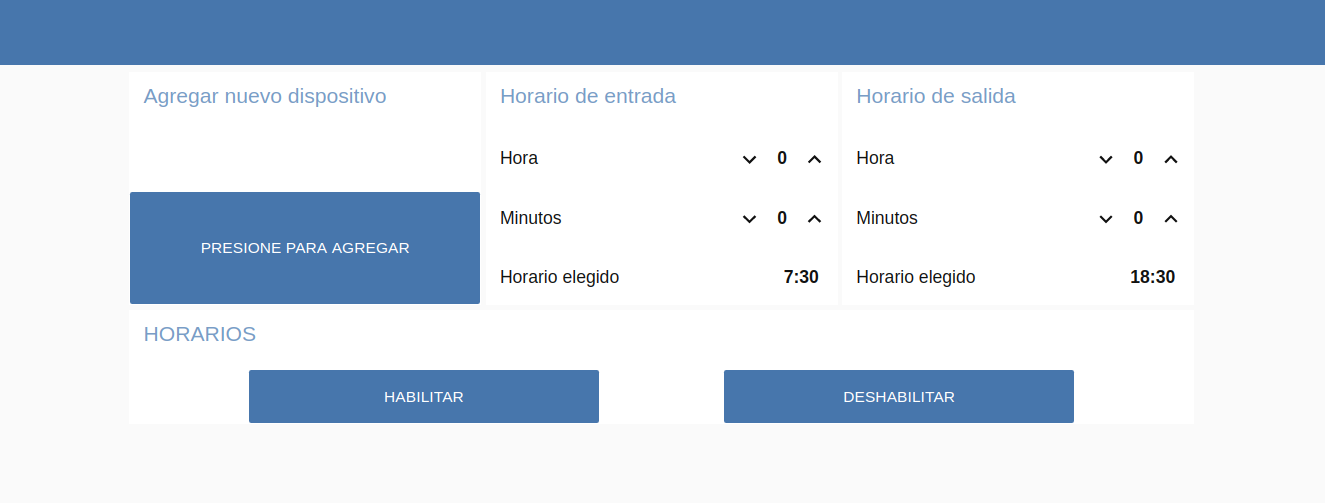
\includegraphics[width=1\textwidth]{./Figures/configuracion.png}
	\caption{Pestaña de configuración de la interfaz web.}
	\label{fig:configuracion}
\end{figure}

La pestaña de reset se puede ver en la figura [\ref{fig:reset}]. Luego de un reseteo del gateway o apagón el sistema no se reestablece automáticamente. Ésta opción fue agregada para casos en los que se necesite intentar conectar todos los nodos que se encuentran en la base de datos en el caso de que alguno se reinicie por algún motivo. Una vez que se presiona el botón de reset, el gateway suspende los hilos que están en proceso y comienza a enviar un comando a cada nodo de la base de datos para conectarlo nuevamente al sistema.

\begin{figure}[t!]
	\centering
	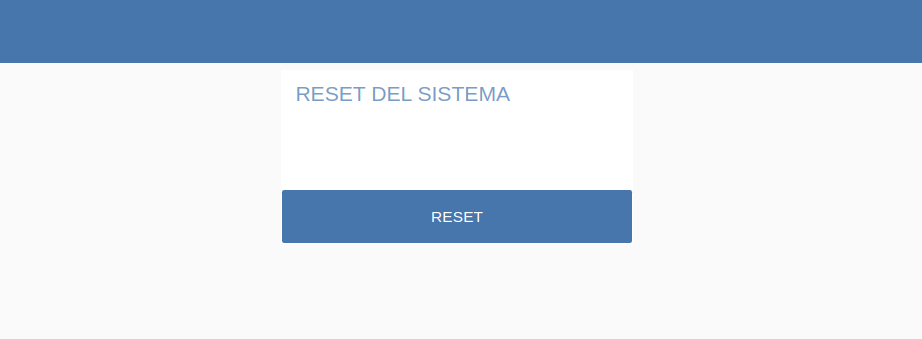
\includegraphics[width=1\textwidth]{./Figures/reset.png}
	\caption{Pestaña de reset de la interfaz web.}
	\label{fig:reset}
\end{figure}
